\documentclass{article}
\usepackage[utf8]{inputenc}
\usepackage[spanish]{babel}
\usepackage{listings}
\usepackage{graphicx}
\graphicspath{ {images/} }
\usepackage{cite}
\usepackage{float}

\begin{document}

\begin{titlepage}
    \begin{center}
        \vspace*{1cm}
            
        \Huge
        \textbf{Proyecto Final}
        
            
        \vspace{0.5cm}
        \LARGE
        DISEÑO
            
        \vspace{1.5cm}
            
        \textbf{Luis Fernando Torres Torres\\Johan David Rojas Martinez}
        
        \vspace{4cm}
            
        \textbf{PhD. Augusto Salazar Jiménez}
            
        \vfill
            
        \vspace{0.8cm}
            
        \Large
        Despartamento de Ingeniería Electrónica y Telecomunicaciones\\
        Universidad de Antioquia\\
        Medellín\\
        Octubre de 2021
            
    \end{center}
\end{titlepage}

\tableofcontents%Tabla de contenidos 
\newpage

\section{Desripción principal}\label{Descripcion}
\noindent
En este informe presentaremos el diseño de nuestro proyecto como las clases y la forma en que interactuan enrtre sí, por otro lado tambien encontraremos un cronocrama que es donde se irá detallando la planificación semana a semana para el desarrollo del videojuego. 
El proyecto se trata de un video juego desarrollado en el lenguaje C++ utilizando el framework de Qt y aplicando la programación orientada a objetos, el videojuego a realizar estará basado en la conocida caricatura infantil Tom y Jerry. 

\section{Modelamiento de los objetos} \label{ideas}
\noindent
En esta sección se da una descripción de las clases que se implementan para la realización del juego, además se coloca los psibles métodos que pueden tener y su relación con distantas partes del programa (forms u otras clases).Para este caso las clases a implementar son 7, donde cada una cuenta con una función distinta y son de vital importancia para el juego, la clases son las siguientes:\\


\noindent\textbf{CLASES}:\
\begin{itemize}

\item\noindent\textbf{mostrarInformación}: 
Esta es una clase la cual  tiene la función de mostrar a los usuarios del juego los controles y teclas que se van a usar para jugar. Esta clase va directamente asociada con un botón que esta colocado en en la ventana principal del juego,también tendra su propio Form denominado informacion.ui, en donde se colocaran todas las imagenes necesarias para dar las instrucciónes de como jugar. En esta clase se implementa únicamente un método que es dar click para salir de la ventana información y continuar para poder jugar.\\ 


\item\noindent\textbf{mostrarEnemigo} : 
Esta clase tiene todos los audios e imagenes que tienen los enemigos, en este caso "Spike" el perro Bulldog de la serie animada Tom y Jerry. Esta clase va asociada con un botón que tiene como objetivo mostrar al usuario del juego toda la información sobre la dinámica de funcionamiento del perro. Como métodos esta clase tiene algunos que permiten  visualizar como es cada uno de los enemigos y ibjetos que generan perdidas de vida.\\

\item\noindent\textbf{menú}: 
En esta clase se coloca se carga la música y las imagenes del juego antes de iniciar. Se da a escoger la opción para jugador único o multijugador, ademas se colocan los botones para información y mostrarEnemigos. Los métodos que van asociados a esta clase son todos aquellos que hacen llamada a las diferentes opciones del juego, donde a su vez se inicializan todas los contenedores que guardan a los enemigos, obstaculos y personajes del juego, Además se inicializa el archivo donde se guardan los datos de las personas que estan jugando y su puntaje.\\
 
\item\noindent\textbf{Obstaculo}: 
Esta clase será utilizada para simular e interactuar con obstaculos a lo largo del juego ya sea para aumentar las vidas o disminuir en caso que colisione con obstaculos enemigos, también se encarga de mover los enemigos y los objetos que colisionarán con el personaje de forma aleatoria. 
Por ejemplo, para aumentar las vidas el personaje debe colisinar con objetos como pedazos de queso, hamburguesas, u otro tipo de comida.
En el caso de que el personaje colisione con huesos que son lanzados aleatoriamente en forma de movimiento parabolico u otros objetos que se mueven en un tipo de movimiento definido en el marco de los requerimientos y a a su vez sea enemigo hará que este pierda vidas.
por otro lado,  tendremos como obstaculo el enemigo que será el BullDog que aparece en la caricatura(llamado Spike), este irá caminando aleatoriamente en direccion contraria a la del jugador, si este colisiona con el BullDog también disminuirán sus vidas debido a que este es un enemigo.\\
 
 
\item\noindent\textbf{personaje}:
Esta clase se encarga de crear objetos de tipo personaje, los cuales actuarán a lo largo de la escena, el personaje podrá moverse en la direccion que le ordene el jugador con movimiento rectilineo,en esta clase se carcagarán y se mostrarán en la posición que ocurra el evento y con una velocidad establecida las imágenes que correspondan a la situación que ocurra en ese instante en la escena, ya sea un choque, una muerte, etc.\\ 

\item\noindent\textbf{resultados}:
Esta clase será utilizada para mostrar en pantalla al jugador o a  los jugadores en el caso de que sea jugado en modo multijugador quien ganó y con cuanto puntaje ganó la partida, distancia recorrida, etc. Esto será mostrado cargando una imagen con decoración para que le de una mejor perspectiva al juego. Aprovechando que esto será utilizado al final del juego también será utilizado para reorganizar, ocultar y mostrar valores, como puntaje de vidas, distancia, entre otros.\\
 
\item\noindent\textbf{seleccionarPersonaje}:
Esta clase será utilizada para que el jugador por medio del mouse, seleccione con cual personaje del juego desea jugar, los dos personajes entre los que puede escoger el jugador son Tom o Jerry, la ventana tendrá un boton para seleccionar el personaje y empezar a jugar. Tambien se aprovecha para poner algo de sonido introductorio caracteristico de la caricatura mientras el jugador decide con cual personaje quedarse. \\
\end{itemize}

\section{Planificación}
\noindent En esta sección se realiza un cronograma de tareas, el cual es una guia que tiene el objetivo de de llevar el control de actividades que se deben desarrollar y tener hechas para una semana definida, en este caso las 2 semanas de trabajo que quedan faltantes. El cronograma planteado por el equipo de trabajo es el siguiente:\ref{f2}

\begin{figure}[h!]
    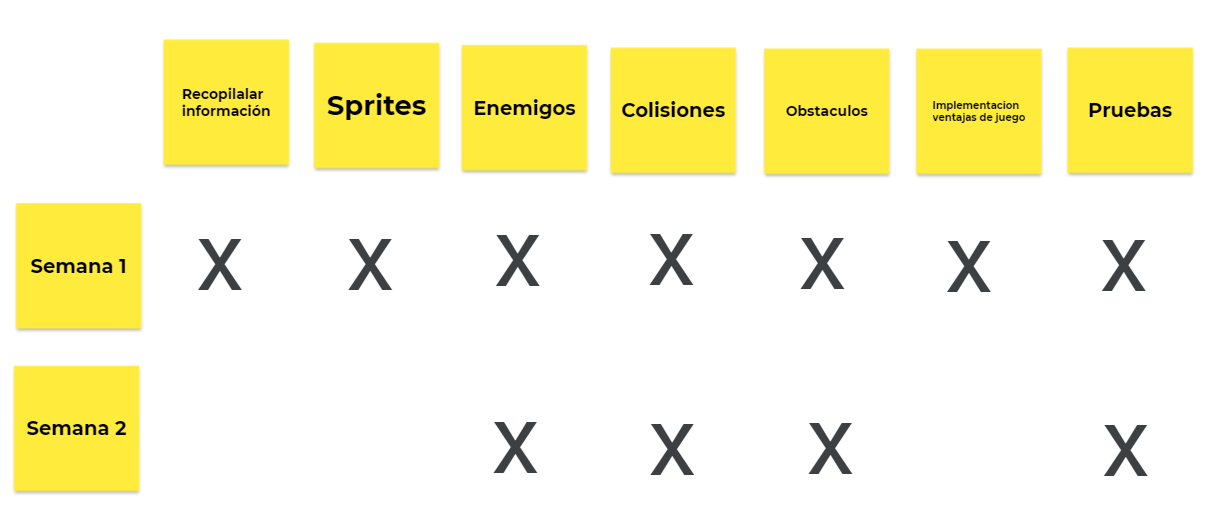
\includegraphics[width=14cm]{Semana1y2.PNG}
    \centering
    \caption{Cronograma de actividades}
    \label{f2}
    \end{figure}

\end{document}